\section{Сила Ампера}

\begin{ex}
\hspace{0pt} \\
\begin{minipage}{.65\textwidth}
(2016) На рисунке представлена модель электродвигателя. Замкнутый контур образован двумя вертикальными рейками, между концами которых включен источник постоянного тока с ЭДС {\Large $\varepsilon$}, a другие концы замкнуты перемычкой сопротивлением $R$ и длиной $L$. Перемычка за счет скользящих контактов может без трения скользить вдоль реек. Контур находится в однородном магнитном поле с индукцией $B$, направленной горизонтально. Известно, что если к перемычке подвесить груз массы $M$, она будет в состоянии равновесия. 1) Определите массу $m$ перемычки. 2) Определите установившуюся скорость ненагруженной перемычки. Сопротивлением реек и внутренним сопротивлением источника пренебречь.
\end{minipage}
\begin{minipage}{.35\textwidth}
\centering
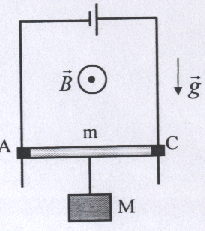
\includegraphics[width = 0.9 \textwidth]{RodInMagneticField.png}
\end{minipage}
\begin{ans}
\end{ans}
\end{ex}

\begin{ex}
(2003) Металлический стержень массой $m$ и длиной $L$ подвешен на двух легких проводах длиной $l$ в магнитном поле с индукцией $B$, 
вектор которой направлен вертикально. К точкам крепления проводов подключен конденсатор емкостью $C$, заряженный до напряжения $U$. 
Сопротивление стержня и проводов пренебрежимо мало. Найти максимальный угол отклонения проводов от вертикали, если разрядка конденсатора происходит за очень малое время.
\begin{ans}
\end{ans}
\end{ex}

\begin{ex}
\hspace{0pt} \\
\begin{minipage}{.65\textwidth}
(2010) Посередине между двумя жестко закрепленными проводниками с током на расстоянии $a$ расположен груз массы $m$, представляющий собой цилиндрическую железную трубку длиной $l_1$ и укрепленный с помощью упругих растяжек длиной $l$. 
Магнитная проницаемость железа $\mu$. Внутри растяжек установлен еще один проводник. По всем трем проводникам течет ток $J$. 
Определите собственную частоту свободных колебаний груза, считая, что в процессе колебаний натяжение растяжек $T_0$ не изменяется. 
Определить зависимость критического значения силы тока от натяжения растяжек, считая критическим значением такое значение, при котором колебания в системе невозможны.
\end{minipage}
\begin{minipage}{.35\textwidth}
\centering
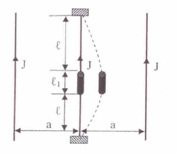
\includegraphics[width = 0.9 \textwidth]{122010AmperesForceLawTwoConductors.jpg}
\end{minipage}
\begin{ans}
\end{ans}
\end{ex}

\begin{ex}
\hspace{0pt} \\
\begin{minipage}{.65\textwidth}
(2017) Одна из моделей генератора постоянного тока представляет собой проводящий диск, который вращается в однородном магнитном поле с индукцией,
направленной перпендикулярно плоскости вращения диска. Если концы некоторого проводника сопротивлением $R$ присоединить к центру диска и через скользящий контакт к его ободу, то в цепи возникнет электрический ток. 1) Объясните
возникновение электрического тока и найдите силу тока, если радиус диска $r = 10$ см, частота вращения диска $\nu = 40$ об/с, индукция магнитного поля $B = 0,1$ Тл, сопротивление нагрузки $R = 0,5$ Ом. 2) Какая мощность затрачивается для поддержания вращения диска? 3) Какой момент силы относительно оси вращения нужно прикладывать к диску? Сопротивлениями диска и контактов пренебречь.
\end{minipage}
\begin{minipage}{.35\textwidth}
\centering
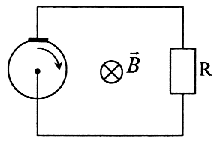
\includegraphics[width = 0.9 \textwidth]{AmperGenerator.png}
\end{minipage}
\begin{ans}
\end{ans}
\end{ex}

\section{Закон Био-Савара-Лапласа}

\begin{ex}
Ток $I$ течет по длинному прямому проводнику, сечение которого имеет форму тонкого полукольца радиуса $R$. Найти магнитную индукцию на оси~$O$.
\begin{ans}
\end{ans}
\end{ex}

\begin{ex}
\hspace{0pt} \\
\begin{minipage}{.65\textwidth}
Найти модуль и направление силы, действующей на единицу длины тонкого проводника с током $I$ в точке $O$, если проводник изогнут так, как показано на рисунке.
\end{minipage}
\begin{minipage}{.35\textwidth}
\centering
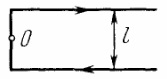
\includegraphics[width = 0.9 \textwidth]{1202BiotSavartLawConductor.jpg}
\end{minipage}
\begin{ans}
\end{ans}
\end{ex}

\section{Теорема о циркуляции индукции магнитного поля}

%Ижевск
\begin{ex}
\hspace{0pt} \\
\begin{minipage}{.65\textwidth}
Однородный диэлектрический диск массой $m$ радиуса $R$, равномерно заряженный с полным зарядом $q$, помещен в однородное магнитное поле с индукцией $B$. Какую угловую скорость получит диск, если выключить магнитное поле?
\end{minipage}
\begin{minipage}{.35\textwidth}
\centering
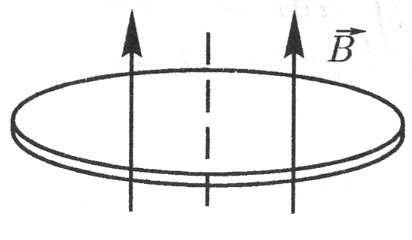
\includegraphics[width = 0.9 \textwidth]{1205AmperesCircuitalLawDisc.jpg}
\end{minipage}
\begin{ans}
\end{ans}
\end{ex}

%Ижевск
\begin{ex}
\hspace{0pt} \\
\begin{minipage}{.65\textwidth}
По поверхности жесткой непроводящей однородной сферы массой $m$ равномерно распределен заряд $q$. 
Сфера может свободно вращаться вокруг своей вертикальной оси. В начальный момент сфера покоилась, а магнитное поле было равно нулю. 
Найти, как меняется со временем угловая скорость сферы при включении однородного магнитного поля, 
сонаправленного с осью вращения сферы и меняющегося во времени по заданному закону $B(t)$.
\end{minipage}
\begin{minipage}{.35\textwidth}
\centering
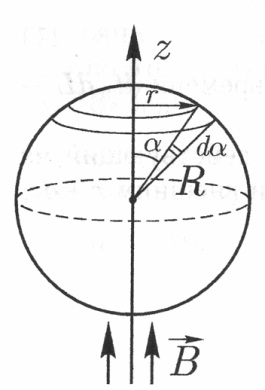
\includegraphics[width = 0.9 \textwidth]{1206AmperesCircuitalLawSphere.jpg}
\end{minipage}
\begin{ans}
\end{ans}
\end{ex}